\chapter{Diffraction in imperfect crystal}
\label{chap:ECCI}

In this chapter we will explore the application of electron diffraction to the study of dislocation lines in the technique known as Electron Channeling Contrast Imaging (ECCI). Before I do that I want to make very sure the reader is on board with the \emph{channelling = diffraction} doctrine.

I will then cover why this is a particularly interesting technique to apply to the world of nitrides where defects are a serious impediment in the improvement of opto-electronic efficiency of devices. 

We mentioned in the previous chapter that the DHW equations can easily accommodate crystallographic information for an introduced dislocation in the form of strain profile. We will have a look at these equations here and how to solve them. Not before we talk about the derivation of the displacement field of a dislocation line and how to project this field on the direction of the incident beam. 


\pagebreak



\section{A word on \textit{channelling}}
\label{sec:channelling}



Centuries after the decline of the Western Roman Empire, the allure of power and honour brought by the title of Roman Emperor was undiminished. While Irene of Athens, a female, was occupying the Roman throne, the pope crowned the king of Franks, Charlemagne, as Holy Roman Emperor -- a new title Charlemagne found nifty enough to add to his already significant collection. But, as Voltaire reflected later on, the title, while maintained for an impressive span of a thousand years, bared little practical significance: ``\textit{[...] the Holy Roman Empire was neither holy, nor Roman, nor an Empire}''. The title persisted even though the territory was not unified in religion and one of the emperors was even excommunicated by the pope. Rome was not by any stretch of imagination the centre of the \textit{Holy Roman Empire}, in fact Italy eventually stopped being part of the empire with no effect on the Empire designation. While its border continued to change, the Holy Roman Empire was consistently made up of Germanic nations. Additionally, Latin was not a popular language across the territories. Finally, unlike the Roman Empire, the Holy Roman Empire was hardly an empire in the sense of unitary legal entity and the absolute power the emperor would hold over its territories. Yet, the name prevailed, despite it being a gross misnomer\footnote{Here is another classic example: the Jerusalem artichoke is the root of a North American plant, in the sunflower family -- the name is probably a corruption of the Italian for ``sunflower'', \textit{girasole}.}, perhaps even an anachronism. 

When it comes to the SEM techniques, their labels are also not terribly accurate. Some keep insisting calling the transmission diffraction  mode in the SEM - transmission electron backscattered diffraction (t-EBSD), apparently oblivious to the oxymoron in the  association. But, perhaps even more confusing, is the fact that, while some techniques carry in their name the type of electron interaction that generates the signal, EBS-Diffraction, TK-Diffraction, others do not. Electron channelling patterns (ECP) and electron channelling contrast imaging (ECP) misleads the inexperienced reader to assume that the source of signal is fundamentally different, that in fact \textit{channelling} might be the type of interaction to blame. These labels are the ``Holy Roman Empire'' of electron microscopy. 

%---------
\begin{figure}[!h]
    \centering
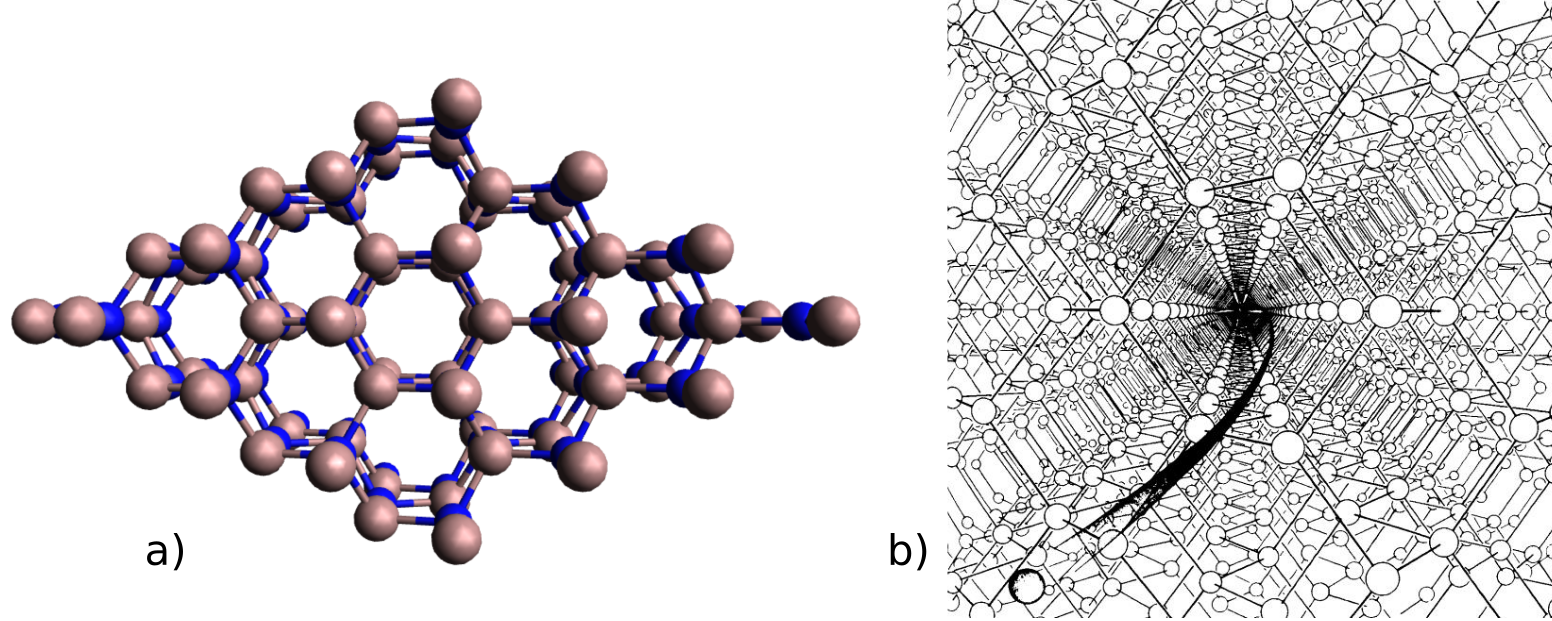
\includegraphics[width=1\linewidth]{Figures/channel2.png}
\caption{ a) Open ``channels'' between rows of atoms along the main direction \hkl[001] in GaN -- \emph{not} responsible for what is sometimes called electron ``channelling''. b) Artist's impression of channelling of heavy charged particles, from~\cite{Brandt68} .}
\label{Fig:channels}
\end{figure}
%---------


These two SEM techniques carry the word \textit{channelling} for historical reasons. In early 1960s, before electrons became widely used in high resolution microscopy, ions were used in much the same way as electrons are in the Scanning Microscope. It was observed that the scattered secondary electron intensity depended on the ions' incident direction~\cite{Davies83}. This was in sharp contradiction with the 
theory of scattering at the time which assumed the distribution of atoms in samples can be approximated to a dense gas. It became apparent that an incident ion beam aligned along any of the major axes of the crystal would yield longer penetration depths, would loose energy slower and would generate fewer secondary electrons close to the surface~\cite{Piercy63}. This was initially explained as simple geometrical transparency, \ie columns of empty space along major axes as shown in Fig.~\ref{Fig:channels} a), such that the ions would simply suffer less scattering on their path as shown in the beautiful artist render in Fig.~\ref{Fig:channels} b) hence the name \textit{channelling}.


Based on these observations, Linhard~\cite{Lindhard65} developed a classical mechanics explanation for incident particles with small and incoherent wavelengths such that effects such as interference patterns can be ignored. He defined the condition for the validity of this classical treatment, more explicitly, through the requirement that the number of bound states in the string potential to be large compared to unity ($\nu_s\gg1$). The full explanation of channelling is somewhat more involved then a simple geometrical transparency. The heavy particles, when incident at a direction close to major crystallographic direction, behave as if focused by total sum potential of the strings of atoms. Correlated deflection by the atoms in the strings protect the incident beam from penetrating close to the core of the atoms and suffer scattering. The resulting effect is that, in these special conditions, the incident particles can travel deeper in the sample and loose less energy, channelling, protected as they are by the potential of the string of atoms. Linhard then went on to establish an  upper limit for stable channelling for the incidence angle relative to a major direction he called the \textit{critical channelling angle}:

\begin{equation}
\theta_{chan} \leq \sqrt{\frac{2 Z e^2}{E d}} 
\end{equation} 
where $Z$ is the atomic number and $E$ is the energy of the incident particle, $e$ is the usual elementary charge and $d$ is the distance between atoms in the string.

Not only strings of atoms but also lattice planes can channel a beam of incident charged particles. In \textit{Notes on Channeling}, Andersen~\cite{Andersen14} explains the qualitative image of planar channelling analogous to the string of atoms channelling. The planar potential can be thought of as a superposition of string potentials, allowing the incident beam particles to sneak in between two strings and still be protected by the deflection of correlated atom scattering. The dark spot in the centre of the angular flux distribution in  Fig.~\ref{Fig:icp} a) is due to lower scattering rates along the direction parallel to the \hkl[001] axis, or string channelling. The dark lines are the result of planar channelling in the family of planes \hkl{100} and \hkl{110}.    


%---------
\begin{figure}[!h]
    \centering
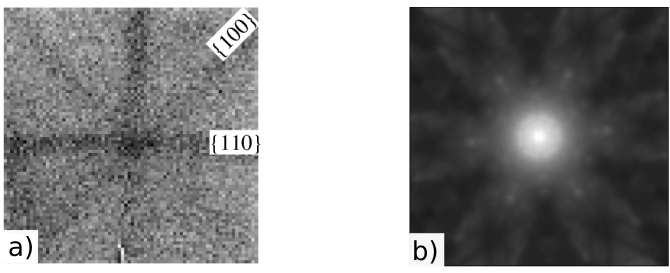
\includegraphics[width=0.66\linewidth]{Figures/icp-ecp.png}
\caption{ a) Flux distribution of heavy C ions scattered from a transmitted beam through \hkl[001] Si crystal, from~\cite{Assmann99}. b) Simulated ECP pattern of \hkl[001] GaN using EMsoft~\cite{EMsoft}. While the observed features are similar, a)~is an effect of channelling and b)~of diffraction.}
\label{Fig:icp}
\end{figure}
%---------





It was soon observed that the channelling extends to other charged particles like high energy protons~\cite{Dearnaley68} or alpha particles. For electrons and positrons, the first indications of crystal lattice influence on the scattering directions was given by observing emission of $\beta$ doped samples~\cite{Uggerhoj68}. It appeared that the scattered yield of increased when electrons were travelling along a lattice direction. These observations were later confirmed by Rutherford scattering experiments of fast electrons incident on a sample~\cite{Uggerhoj69}. It was only natural to make the parallel with ions scattering experiment and call the phenomena \textit{channelling}.  

Mysterious is the fact that Coates had already published, two years previously, his observation of Kikuchi like patterns in the SEM~\cite{Coates67} -- bright lines of increased electron backscatter intensity associated with lattice planes, yet the connection between the two phenomena was not made. By the time Joy wrote his significant contribution to the description and understanding of directional dependence of scattering in the SEM~\cite{Joy82}, the name of channelling already gained traction and the phenomena was known as Electron Channelling Patterns (ECPs). When comparing the angular distribution of scattered ions (Fig.~\ref{Fig:icp} a) ) with that of electrons (Fig.~\ref{Fig:icp} b) ), the similarities are indeed indisputable. The contrasting lines in both cases are due to the lattice planes. In the first case the lines are dark indicating a lower scattering rate of ions when close to lattice directions and planes. However, in the electron case, the lines are bight indicating an increase in scattering when electrons are close to the planes or directions. 

For a polycrystalline sample, the contrast in intensity from one grain to the other seems similar when using ions~\cite{Franklin88} and electrons. Since for ions it was attributed to channelling it only made sense to blame channelling for change in electron yield (contrast) for different orientation grains (Electron Channelling Contrast Imaging). When we say electron channelling we only mean channelling in the sense of a stable trajectory close to atoms and planes. Nevertheless, the underlying physics is different. 

\begin{table}[h]
\caption{Critical channelling angle $\theta_{chan}$ and Bragg angle $\theta_B$ for heavy C ions and electrons travelling along \hkl(001) planes in a GaN sample. The number of bound states for strings $\nu_s$ and planes $\nu_s$ indicate the validity of the classical description of channelling. }
\label{table:channelling}
\centering
\begin{tabular}{ l l c c c c }
\toprule
\tabhead{Particle} & \tabhead{Energy [\si{\mega \electronvolt}]} & \tabhead{$\nu_s$ (classical?)} & \tabhead{$\nu_p$ (classical?)} & \tabhead{$\theta^{chan}$ [\si{\degree}]} & \tabhead{$\theta_B$ [\si{\degree}]} \\
\midrule
  C ion     &  1     & $>10$ (yes)            & $>10$ (yes) & $\leq 1.2 $           & $\leq 10^{-4}$\\
  electron  &  1     & $\approx 4$ (uncertain)& $< 1$ (no)  & $\leq$ \textit{0.1}   & $< 0.1$ \\
  electron  &  0.02  & $< 1$ (no)             & $< 1$ (no)  & $\leq$ \textit{0.9}   & 0.5\\
\bottomrule
\end{tabular}
\end{table}

For MeV ions, with short wavelengths, the interference effects can be safely ignored since mean free path for inelastic scattering is as sort as a few lattice spacings. Meanwhile, for fast electron we cannot ignore that at Bragg angles their scatter amplitude will interfere constructively which is what gives the strong, sharp peak in the scattered yield. The legitimacy of a classical description, such as channelling, for explaining these peaks is, nevertheless, doubtful. 




In Table~\ref{table:channelling} I calculated the number of bound states, for both strings of atoms ($\nu_s$) and planes ($\nu_p$), for electrons at \SI{1}{\mega \electronvolt} and \SI{20}{\kilo \electronvolt} scattered along \hkl(001) planes in GaN. For electrons, the number of bound states in the string potential can be reduced from~\cite{Lindhard65} to:
\begin{equation*}
\nu_s \approx \frac{1}{\sqrt{1-\frac{v^2}{c^2}}}\,\, Z^{1/3} \,\, \frac{4a_0}{d}
\end{equation*}
and the number of bound states in a planar potential to:
\begin{equation*}
\nu_p \approx \frac{0.4}{(1-\frac{v^2}{c^2})^{1/4}} 
\end{equation*}
where $Z$ is the atomic number of the target material, $a_0$ is the Bohr radius, $d$ is the distance between atoms in a string and $v$ is the speed of the incident particle~\cite{Uggerhoj69}.  

Diffraction and channelling are two separate but competing phenomena. They are defined by the channelling angle and Bragg angle, respectively, and looking at the range of these parameters we can decide which of these events dominates. For electrons with energies below \SI{1}{\mega \electronvolt} the classical description is not appropriate, and the critical channelling angle is meaningless, which is why I wrote it in italic. But very high energy electrons with energies above \SI{1}{\mega \electronvolt} channelling can become a relevant phenomena and will compete with the Bragg angle. We can see the situation is reversed for heavy ions, which are highly localised with numerous bound states, both in the string potential and the planar potential. However, the Bragg angle is vanishingly small for these heavy particles and therefore diffraction effects can be ignored. 

For SEM electron energies we are comfortable in the non-channelling range. Nevertheless, we will continue to use Holy-Roman-Empire-names of Electron Channelling Pattern and Electron Channelling Contrast Imaging and understand that the word channelling in these cases is different from the effect of ions channelling, referring instead to stable trajectories close to atomic nuclei for the electron Bloch waves. 






\section{Why study TDs in nitrides using electron diffraction?}

Over the past thirty years there has been no shortage of interest in electronic and light emitting devices based on semiconductors and, as a result, their impact on modern technologies has become notable. Brighter, more efficient and more reliable light sources have been developed. Additionally, we have witnessed an ever increasing  span of other emerging applications: from ultraviolet light water purification and hydrogen production to high power electronics and novel optical communication systems. The bottleneck of developing the next generation devices remains the material science of improving even further the efficiency for these devices.

The group III-nitride material systems and their alloys have been intensely studied due to a number of promising properties. The large difference in covalent bondings of the elements in these III-V systems translates to greatly varying physical properties, including different lattice parameters and energy band gaps. The later means that nitride alloy systems can offer a wide range of direct energy-band gaps, \ie high intensity luminescence at a wide range of wavelengths (\eg the band gap of InAlGaN systems ranges from infrared to the ultraviolet region).  In addition, their stability at high temperatures and good thermal conductivity make them ideal candidates for the fabrication of high power transistors. GaN is one such binary system and together with its cousins, InN and AlN, and their ternaries and quaternary alloys are one of the semiconductors on top of material scientists minds, after Si and Ge, due to their many applications in optical and electrical devices.  

Nevertheless, unlike Si and Ge, the group III nitrides epitaxial growth is challenging due to the lack of a suitably lattice matched material. The lattice mismatch can be significant and the usual compromise between cost and growth impairment is sapphire ($Al_2O_3$), which at room temperature and along the r-plane has a lattice mismatch of $\sim1.1\%$~\cite{nitrides} with GaN grown in \hkl[0001] direction. The epitaxial layers will be further strained during the cooling down stage, such that, at the end of the growth process, a thick layer will relax through the formation of misfit dislocations along the interface of lattice mismatched materials.

An interface misfit dislocation introduces a discontinuous strain in the crystalline lattice, and way to resolve the discontinuity is thought the generation of \textit{threading dislocations} (TDs) which run from the layer interface through the crystal up to its surface. Dislocations and line defects of crystalline solids can strongly affect the properties of the material and the performance of the devices we would like to use these materials for.

Surprisingly, the blue emitting devices based on III-nitrides are able to function even in the presence of TDs  densities of the order of $10^{11}$/cm$^2$, due to the carrier localisation effect~\cite{Graham}. However, for a great number of devices, TDs prove to be problematic as they tend to be associated with impaired optical and electrical performances. For example, TDs correlate with increased leakage current in green and blue light emitting diodes (LEDs) \cite{Ferdous} and overall reduction in efficiency in near-UV LEDs~\cite{Kamiyama}. Moreover, TDs can be blamed for reducing the life of laser diodes as well as decreasing the electron mobility in high electron mobility transistors~\cite{Bougrioua}. TDs can cause premature junction breakdowns as well as inhibiting high current gains in GaN based UV avalanche photodiodes~\cite{Limb}. They are also connected to the current collapse in GaN field-effect transistors~\cite{Disanto} and the general degradation in performance of high power GaN based devices. It therefore becomes apparent the need to study the origin, development and impact of TDs in order to perfect growth methods aimed at reducing the TDs density.



%-------
\begin{figure}
\centering
\noindent\begin{minipage}{0.47\textwidth}
    \centering
    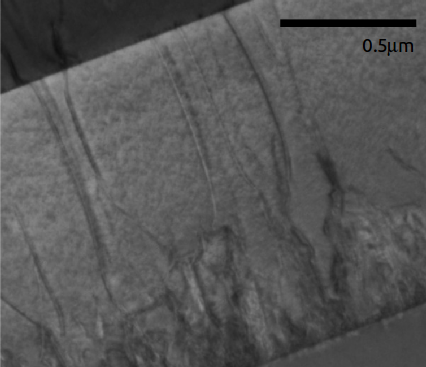
\includegraphics[width=0.9\linewidth, height=0.25\textheight]{Figures/TEM.png}
    \captionsetup{width=0.8\linewidth}
    \caption[magic]{Transversal TEM image\footnote{Taken at the KNC, University of Glasgow. ~~By permission of David Thomson} of an AlGaN on sapphire showing threading dislocations reaching an interface.}
     \label{fig:tem}
\end{minipage}
\;\;\;
\begin{minipage}{0.48\textwidth}
     \centering
     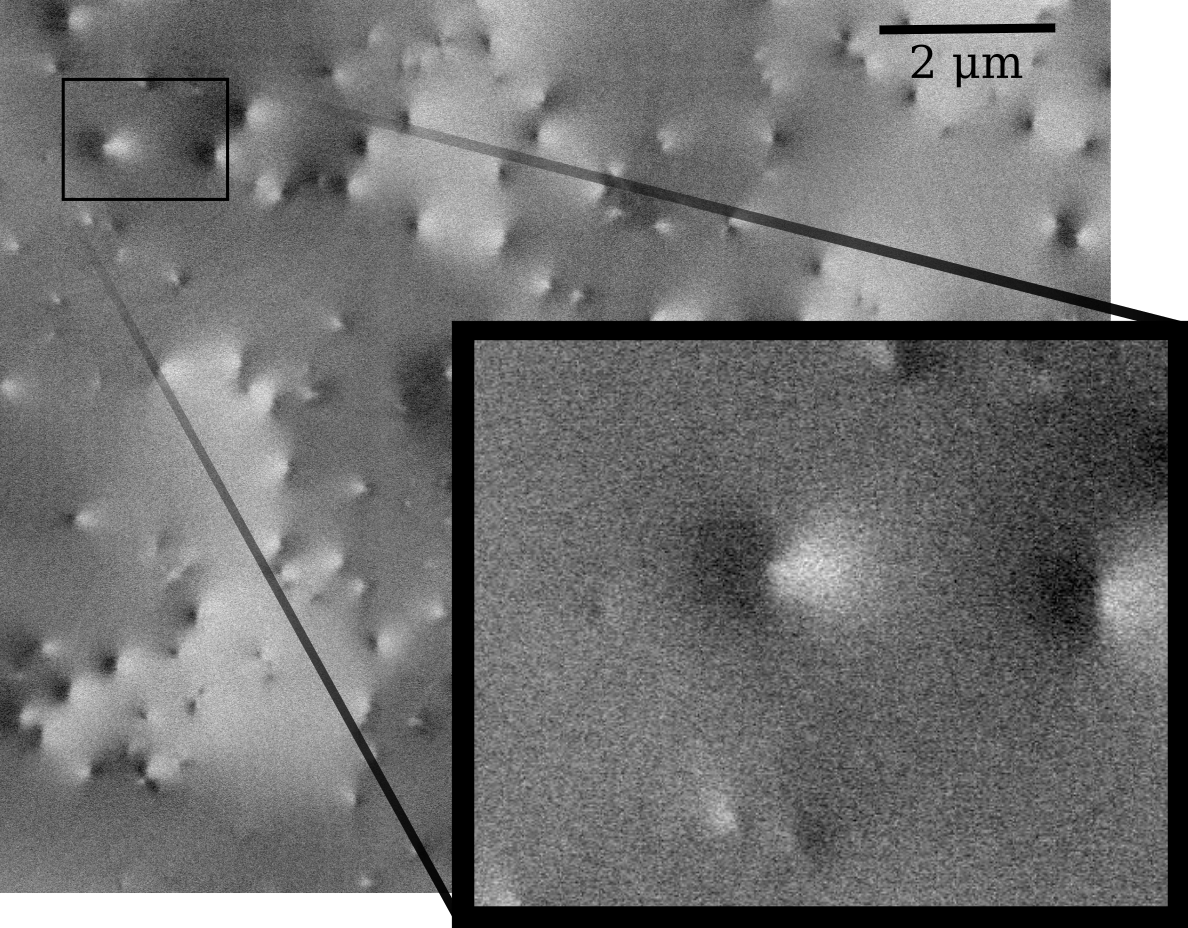
\includegraphics[width=0.9\linewidth, height=0.25\textheight]{Figures/ECCI.png}
      \captionsetup{width=0.8\linewidth}
     \caption[]{Plan view ECC image\footnote{By permission of Allehiani Nouf Mohammad} of a \hkl[0001] GaN on sapphire showing black-white contrast around threading dislocations.}
     \label{fig:ecci}
\end{minipage}
\end{figure}
%---------

Electron diffraction is one mechanism that is sensitive to the presence of strain due to dislocations in the crystal, facilitating therefore dislocation imaging. Transmission electron microscopy (TEM) has established itself as the default technique for the study of lattice
deformations and identify defect types. We will talk more about dislocations in the next section but for now it is useful to know that two extreme \hkl[0001] threading dislocation characters can be distinguished:pure screw type (or \textit{\textbf{c}-type}) where the Burgers vector (\textbf{b}) is aligned along the \textit{c}-axis and pure edge dislocation (or \textit{\textbf{a}-type}) when the Burgers vector is confined to the (0001) basal plane. If neither of these conditions is strictly met, the dislocation is called mixed, or \textit{\textbf{a+c} type}.



TEM is especially reliable as a dislocation characterisation method as it can identify unambiguously the \textbf{c} and \textbf{a} components of a dislocation line running parallel to the imaged surface. This is achieved through the application of certain relationships between the diffraction vector $\vb{g}$, Burgers vector $\mathbf{b}$ and the direction of the dislocation line $\mathbf{u}_l$ ($\vb{g} \cdot \vb{b} = 0$ and $\vb{g} \cdot \vb{b} \times \vb{ u}_l = 0$), known as the \textit{invisibility criteria}, for which no contrast associated
with \textbf{c} or \textbf{a} components can be observed. This method has been applied broadly in the study and
characterisation of dislocations in cross sectional GaN samples (\eg~\cite{Hino00}). For TDs which penetrate the sample surface normally (or almost normally) high resolution TEM (HRTEM) can provide direct observation of the Burgers vector direction of a type TDs. However, as the images are usually acquired in plan view, the \textbf{c} components are invisible. The destructive TEM sample preparation and its limited field of view can also restrict the number of defects that can be observed and hence may impact the statistical limits on estimating defect densities, particularly for materials with lower numbers of dislocations.


There are characterisation methods which do not share TEM’s requirements for sample preparation. These
include atomic force microscopy (AFM), which can offer information on TDs associated with surface pits~\cite{Craven02} (often after an etching or decoration treatment) or when terminating in step edges. However, AFM can be sensitive to surface debris and may require extended period of time to image even relatively small areas~\cite{Koinkar97}. Alternatively, for larger area measurements, X-ray diffraction~\cite{Heinke00} or cathodoluminescence (CL)~\cite{Rosner97} can provide information on the global material defects densities but can have limitations in terms of resolving individual dislocations. 

An alternative to the above methods is the use of electron contrast channelling imaging (ECCI) technique which can be employed within generally available field emission scanning electron microscopes (FE-SEMs). This approach can image defects with resolution of a few nanometers with a micrometer scale field of view, and is neither destructive nor based on direct sample contact. However, in order to obtain the maximum amount of information from these images, a thorough understanding of the contrast mechanisms is required.

Trager-Cowan \etal\cite{Carol} showed that using ECCI in the characterisation of nitrides is an excellent idea. ECCI has been used in the forescatter geometry to reveal extended defects and
morphological features of GaN samples while also delivering information about crystallographic orientation~\cite{Picard}. The electron channelling contrast images obtained in the SEM can provide structural information on dislocations  interacting with the sample surface, particularly when obtained in highly diffracting channelling conditions~\cite{Naresh}. This information is shown in the form of variation in the electron backscattered (BSE) intensity around a dislocation -- or dark-bright signal contrast on the micrograph. Because it can resolve individual dislocations while imaging larger areas (e.g. Nouf-Allehiani et al.~\cite{Nouf} for material with TDs having a mean separation of $\approx$ 200 nm), ECCI is an ideal candidate for both precise and accurate number estimates for a wide range of TD densities (\SI{10e6}{\centi \metre^{-2}} -- \SI{10e10}{\centi \metre^{-2}} ).


 
 \section{Electron channelling modelling???????????}
\todo{Fix me}
Diffraction of high energy electrons traditionally is taken to imply elastic scattering from the understanding of diffraction in TEM. Defect characterisation in TEM is relatively well established. Both qualitative models such as the kinematical theory~\cite{Hirsch60} which only assumes a single scattering process to occur from the direct beam of electrons into the diffracted one, and more quantitative models -- the dynamical theory-- which takes into account multiple scatterings between the two beams~\cite{Howie61} have been developed and broadly applied~\cite{Hirsch60,Clarke71,Spencer72}.

However, for thicker samples than the ones valid for the approximations implied in the above theories, inelastic scattering of electrons also becomes important. This has a twofold implication. On one hand, electrons are ``absorbed" from the diffracted beam(s) through inelastic scattering, and this loss must be accounted for. On the other hand, these inelastically scattered electrons are also responsible for some of the features in the patterns observed in the SEM. If we are to study these features, we require a separate dynamical formulation of the inelastic interactions. If we are interested in a quantitative description of defect contrast for different beam orientations as observed in the ECCI (or over many outgoing beams as in EBSD), we ought to couple the dynamical descriptions of the two electron scattering mechanisms. This has previously been achieved by matching the dynamical theory solution, which accounts for elastic effects, at the entrance surface of the crystal to a multiple scattering theory, developed to account for the inelastic processes, at greater depths inside the crystal\cite{Baines73,Howie78}.

The dynamical theory solves the Schr\"{o}dinger equation for the high energy electrons inside a crystal. The electrons see the perfect crystal as a periodic potential and their wavefunction is perturbed in such a way that if we consider a forward scattered electron wavefunction and a backwards scattered one, the amplitude will be dynamically transferred between these two waves as they travel through the crystal in a manner similar to the transfer of energy in the coupled pendulum oscillations. Figure~\ref{fig:fringes} shows exactly this periodic variation in the direct wave intensity (bright field) with depth in crystal by plotting the measured intensity of the transmitted beam along the bottom of wedge crystal. This thickness fringes are a direct result of the fact that the direct and diffracted electron wave intensities oscillate with depth in the crystal.



Two equivalent quantum mechanical descriptions of the electron wavefunction behaviour inside a crystal are given below:
\begin{enumerate}
\item First, we can treat electrons as optical waves (or beams) $\{\Phi(\textbf{g})\}$\footnote{\textbf{g} is the usual reciprocal lattice vector.} where we consider the incident wave of complex amplitude $\phi_0(z)$  and at least one diffracted beam of complex amplitude $\phi_g(z)$ both of which vary with depth $z$ into the crystal. We usually set the boundary conditions of $\phi_0=1$ and $\phi_g=0$ at the entry surface of the crystal. If the crystal is thin enough we can ignore scattering from the diffracted beam back into the incident one, but if the crystal is thicker we must link together the amplitudes $\phi_0$ and $\phi_g$ through a coupled differential equation of the form \cite{Howie61}:
\begin{equation}
\dfrac{d\phi_0}{dz} =\dfrac{\pi i}{\xi_0}\phi_0+\dfrac{\pi i}{\xi_g}\phi_g \exp(2\pi i s z)\\
\dfrac{d\phi_g}{dz} =\dfrac{\pi i}{\xi_0}\phi_g+\dfrac{\pi i}{\xi_g}\phi_0 \exp(-2\pi i s z)
\end{equation}
where $\xi$ is an important parameter known as the ``extinction distance" which measures the physical distance over which the beam amplitude is scattered back and forth between the beams and $s$ measures the deviation from exact Bragg diffraction\footnote{In reciprocal space the exact Bragg condition requires the lattice points to lie on the Ewald sphere.}.

The equations above are valid for a perfect crystal and also ignores any absorption due to inelastic scattering. However, they can easily be generalised to account for imperfections by adding a vector $\textbf{R}(\textbf{r})$ which measures the deviation from a perfect lattice. The theoretical profile in Figure~\ref{fig:fringes} is not something we would observe in the real microscope where the effect of absorption is important. In reality, the oscillations would also die out with the thickness of the crystal as more and more electrons are removed from the diffracting beam. Nevertheless, we can phenomenologically account for this effect as well. Using an idea borrowed from x-ray diffraction, namely that adding an imaginary part to the electrostatic lattice potential has essentially the same effect as accounting for the electrons lost to inelastic scattering.

\item The second description of the electron wavefunction has to do with the periodicity of the crystal potential. It seems straightforward to take advantage of this periodicity in writing out the description of the electron's wave. In this description the steady state solutions of the wavefunction of the electron inside a periodic potential of the crystal are known as Bloch waves $\{\psi(\textbf{r})\}$. The electron wavefunction inside the crystal obeys the non-relativistic Schr\"{o}dinger's equation\footnote{For an electron beam under an accelerating voltage of 30 kV we can calculate the speed of the electrons to be $\sim(0.1 \times$ speed of light), far outside any important relativistic effects.}:
\begin{equation}
\dfrac{-\hbar^2}{2m}\nabla^2\psi(\textbf{r})+[E+V(\textbf{r})]\psi(\textbf{r})=0
\end{equation}
where the kinetic energy of the electron is related to the wave vector in the usual manner:
$E_{kin}={\hbar^2k^2}/{2m_e}$ and $V(\textbf{r})$ has the periodicity of the crystal lattice (i.e. $V(\textbf{r})=V(\textbf{r}+\textbf{a})$ where \textbf{a} is any lattice vector).
The solution of this equation in the form of Bloch waves of wave vector $\textbf{k}$ is of the form:
\begin{equation}
\psi(\textbf{r})^{(i)}= \sum _g C^{(i)}_g(\textbf{k}^{(i)})\exp(2\pi i(\textbf{k}^{(i)}+\textbf{g})\cdot \textbf{r})
\end{equation}
where $C_g(\textbf{k})$ denotes the wave amplitude of the Bloch wave of wave vector $\textbf{k}$.

The minimum number of Bloch waves we can choose is also two. The first Bloch wave is defined such that its maxima are at interstices, while the second Bloch wave's maxima occur on atom columns. We can also offer a more intuitive picture of the anomalous absorption in this frame since it is to be expected that the electrons from the second Bloch waves, that spend more time near the atomic nuclei will be more readily scattered than the ones contained in the first Bloch wave.
\end{enumerate}

The two descriptions above are equivalent \cite{electronMicroscopy}, such that we can write, after some manipulation:
\begin{equation}
\phi_0(\textbf{r}) =C_0^{(1)}\psi^{(1)}(\textbf{r})+C_0^{(2)}\psi^{(2)}(\textbf{r})\\
\phi_g(\textbf{r}) =C_g^{(1)}\psi^{(1)}(\textbf{r})\exp(i\textbf{g}\cdot \textbf{r})+C_g^{(2)}\psi^{(2)}(\textbf{r})\exp(i\textbf{g}\cdot \textbf{r})
\end{equation}
with the boundary conditions:
\begin{equation}
\phi_0(0) =\sum_{i=1,2}\phi^{(i)}C_0^{(i)}=1 \\
\phi_g(0) =\sum_{i=1,2}\phi^{(i)}C_g^{(i)}=0
\end{equation}

In the case of crystal subject to a deformation that moves an atom from the point $\textbf{r}$ to a point $\textbf{r}+\textbf{R}(\textbf{r})$ the potential of the crystal changes by a factor \{$\exp(-2\pi i \textbf{g}\cdot \textbf{R}(\textbf{r}))$\}. The derivation of the displacement field $\textbf{R}(\textbf{r})$ is the subject of the Section \ref{strain}.

So far we have discussed diffraction, but as previously mentioned, if we are interested in backscattered electrons we must also consider the behaviour of the inelastically scattered electrons. Approaches including multiple inelastic scattering calculated out of transport type equations\cite{Spencer72, Spencer80} have been incorporated into diffraction theories in order to produce a more quantitative description of the backscattered electrons intensities. This type of approach has then been implemented in order to predict contrast profiles for dislocation lines running parallel to the crystal surface (i.e. misfit type dislocations) for both screw~\cite{Spencer72} and edge dislocations~\cite{Wilkinson95}. However, no attempts had been made so far to apply this approach to threading dislocation and more importantly to threading dislocations reaching the surface.


 
 \section{TDs strain field in backscatter SEM}
 \todo{fix Strain}
 As part of continuum mechanics, elasticity theory ignores the fact that matter is made out of discrete particles and instead approximates it to be continuous and uniform even at the microscopic level. This conveniently enables us to ignore the very complicated interaction between the many atoms as well as any discontinuing properties at the microscopic level (including the actual dislocations!) simplifying the treatment a great deal. Instead, it entertains the more intuitive idea that matter fills the entire region of space it occupies in a continuous and homogeneous manner and that this holds true for any infinitesimal region of space. While this is not a rigorous description at the microscopic scale, for the micrometer level study of structural effects of dislocations, these crude assumptions will hold fully.

In this model all the specific physical properties of the continuum are exactly the same for
any infinitesimal selected region. This facilitates the substitution of what would otherwise be discontinuous quantities with single valued, smooth fields representing the average value over that infinitesimal region of space of the property we would want to study. This is a useful trick because it allows us to use calculus and treat these properties of interest as tensors well defined at any point in space.

%-------
\begin{figure}[h]
    \centering
    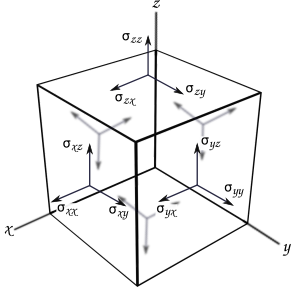
\includegraphics[width=0.39\linewidth, height=0.24\textheight]{Figures/cubefin.png}
    \caption{Stress distribution on an infinitesimal volume.}
    \label{fig:stress}
\end{figure}
%---------

Within the framework of continuum mechanics we also make the assumptions of \textit{linearity} and \textit{perfect elasticity}. The final approximation we will introduce is that of \textit{elastic isotropy}. We provide below the implications of these assumptions:
\begin{enumerate}
\item If a body returns to its original form completely after any deformation force is applied, we say that object posses the property of \textit{perfect elasticity}. Mathematically this is achieved by keeping the forces that produce the deformation below the plasticity region of the structural material of interest, or in other words very small (small enough).

If we define $\sigma_{ij}$ as the $i^{th}$ component of the stress (force per unit area) on a plane whose normal is in the $x_{j}$ direction as shown in Figure~\ref{fig:stress}, and then consider that when acted upon by stress a body deforms such that the displacement at point \textbf{r} is \textbf{u} with component $u_{i}$ we can define strain as:
\begin{equation}
\epsilon_{ij}=\dfrac{1}{2}\left(\dfrac{\partial u_i}{\partial x_j} + \dfrac{\partial u_j}{\partial x_i}\right)
\end{equation}

\item In the equation above we have assumed the distortions are small enough that we can ignore all but first terms in the expansions of individual displacement components. This is also known as \textit{linearity} and also produces a linear relation between stresses and deformations (Hooke's law):
\begin{equation}
\sigma_{ij}=c_{ijkl}\epsilon_{kl}
\end{equation}
where the coefficients $c_{ijkl}$ are the elastic constants which for the most general case form a 9x9 matrix relating the nine elements of $\sigma_{ij}$ to the nine elements of $\epsilon_{kl}$.

\item The final assumption we make here is to state that our material can be reduced to \textit{elastic isotropy} without impairing greatly the accuracy of the results. This is the property of a material whose elastic properties are independent on the orientation we study it in. This in general is not the case for none but a handful of cubic structure, which is it constitutes the main approximation of the present model and we shall always quantify how far away from this the real material is.
\end{enumerate}

Taking into account isotropy reduces the $\{c_{ijkl}\}$ elastic constant matrix from 9x9 elements to only two independent constant and we can rewrite equation (7) as:

\begin{equation}
\begin{bmatrix}
\sigma_{11}\\
\sigma_{22}\\
\sigma_{33}\\
\sigma_{23}\\
\sigma_{13}\\
\sigma_{12}
\end{bmatrix}
=
\begin{bmatrix}
2\mu+\lambda  &  \lambda       &  \lambda       &  0 & 0 & 0\\
\lambda       &  2\mu+\lambda  &  \lambda       &  0 & 0 & 0\\
\lambda       &       \lambda  &  2\mu+\lambda  &  0 & 0 & 0\\
 0            &       0        &  0             &\mu & 0 & 0\\
 0            &       0        &  0             &0   &\mu& 0\\
 0            &       0        &  0             &0   & 0 & \mu
\end{bmatrix}
%
\begin{bmatrix}
\epsilon_{11}\\
\epsilon_{22}\\
\epsilon_{33}\\
2\epsilon_{23}\\
2\epsilon_{13}\\
2\epsilon_{12}
\end{bmatrix}
\end{equation}
with $\mu$ known as the shear modulus and $\lambda$ the Lam\'{e} constant.

 
 \subsection{Surface effects}
 For a screw dislocation the relaxation displacements in Cartesian coordinates with the notation from \cite{Indenbom} are simply:
\begin{align}
u_x =& \dfrac{b}{2\pi}\dfrac{y}{r-z}\\
u_y =& -\dfrac{b}{2\pi}\dfrac{x}{r-z}
\end{align}

In the case of an edge dislocation the relaxation displacements are given in Cartesian coordinates in the notation from \cite{Indenbom} as:
\begin{align}
u_x =& \dfrac{\nu b}{4 \pi(1-\nu)} \left[\dfrac{2xyz}{r(r-z)^2}+(1-2\nu)\dfrac{xy}{(r-z)^2}\right] \\
u_y =& \dfrac{\nu b}{4 \pi(1-\nu)} \left[(1-2\nu)\log(r-z) - (3-2\nu)\dfrac{z}{r-z} + (3-2\nu)\dfrac{y^2}{(r-z)^2} - \dfrac{2y^2}{r(r-z)}\right] \\
u_z =& \dfrac{\nu b y}{2\pi(1-\nu)} \left[\dfrac{1}{r} + (1-2\nu)\dfrac{1}{r-z}\right]
\end{align}